\section{Preliminary Knowledge}
This chapter explains the basics of qubits, quantum gates, and quantum circuits.
%% \begin{figure}[t]
%%   \begin{minipage}[t]{.22\textwidth}
%%     \centering
%%     \scalebox{1.0}{
%%       \Qcircuit @C=0.5em @R=0.2em @!R { \\
  \lstick{\ket{x}} & \qw & \ctrl{1} & \qw & \rstick{\ket{x}} \\
  \lstick{\ket{y}} & \qw & \targ    & \qw & \rstick{\ket{x \oplus y}}  \\
}


%%     }
%%     \subcaption{CNOT-gate}
%%     \sublabel{fig-cnot}
%%     \centering
%%     \scalebox{1.0} {
%%       \Qcircuit @C=0.5em @R=0.2em @!R { \\
  \lstick{\ket{x}} &\qw & \gate{T}    & \qw & \rstick{e^{i\frac{\pi}{4}x}\ket{x}}  
}


%%     }
%%     \subcaption{T-gate}
%%     \sublabel{fig-tgate}
%%     \centering
%%     \scalebox{1.0} {
%%       \Qcircuit @C=0.5em @R=0.2em @!R { \\
  \lstick{\ket{x}} & \qw & \targ    & \qw & \rstick{\ket{\bar{x}}}
}


%%     }
%%     \subcaption{NOT gate}
%%     \sublabel{fig-notgate}
%%   \end{minipage}
%%   \begin{minipage}[t]{.22\textwidth}
%%     \vspace{5mm}
%%     \centering
%%     \hspace{5mm}
%%     \centering
%%     \scalebox{1.0} {
%%       \Qcircuit @C=0.5em @R=0.2em @!R { \\
  \lstick{\ket{x}} & \qw & \gate{H}    & \qw & \rstick{\frac{1}{\sqrt{2}} (\ket{0} + {(-1)}^{x}\ket{1})}  
}


%%     }
%%     \subcaption{H-gate}
%%     \sublabel{fig-hgate}
%%     \centering
%%     \scalebox{1.0} {
%%       \Qcircuit @C=0.5em @R=0.2em @!R { \\
  \lstick{\ket{x}} & \qw & \gate{T^{\dagger}}    & \qw & \rstick{e^{-i\frac{\pi}{4}x}\ket{x}}  
}


%%     }
%%     \subcaption{$T^{\dagger}$-gate}
%%     \sublabel{fig-tdgate}
%%   \end{minipage}
%%   \caption{\blueout{The H, CNOT, T , NOT gates}}
%%   \label{fig-basis}
%% \end{figure}

\subsection{Quantum Gates and Quantum Circuits}
\label{Subsec:qubits}
Quantum computers internally represent data as \emph{qubits}, which are quantum systems that can
take on the states $\ket{0}$ and $\ket{1}$.  We can combine these qubits into bit strings to
create multi-qubit states. In particular, there exists a specific set of these called
\emph{computational basis states} which are of the form $\ket{x_0}\otimes\ket{x_1}\otimes\cdots\otimes\ket{x_{n-1}}=\ket{\mathbf{x}}$ where $x_{0}x_{1}\cdots{x_{n-1}}=\mathbf{x}$, for $\mathbf{x} \in \{0,1\}^n$,
where $n$ is the number of qubits in the system, and $\otimes$ is tensor multiplication between quantum states~\cite{nielsen2010quantum}. These computational basis states
can in turn be used in linear combination to express a generalized quantum state
$\ket{\psi} = \sum_{k \in [0,1]^n} e^{i {\theta}(\mathbf{k})} \ket{\mathbf{k}}, \mathbf{k} \in \{0,1\}^n$, where ${\theta}(\mathbf{k})\in [-\pi,\pi]$ is
an arbitrary phase that is a function of $k$. 

\emph{Quantum gates} map quantum states $\ket{\psi} = \sum_{k \in [0,1]^n} e^{i {\theta}(k)} \ket{k}$ to
other quantum states $\ket{\phi} = \sum_{j \in [0,1]^n} e^{i {\theta}(j)} \ket{j}$.

%We describe their behavior in Fig. \ref{fig-basis}. 

In this paper, we consider the elementary gate set consisting of the $H$-gate, $\mathit{CNOT}$, $T$-gate, $T^{\dagger}$-gate  (the inverse of the $T$-gate), and $NOT$-gate. In the fault-tolerant paradigm, $T$-gates and $T^{\dagger}$-gates are much more expensive to implement than
$H$-gate, $CNOT$, and $NOT$-gates. Hereafter, we will refer to the set of the T-gate and the T$^{\dagger}$-gate as ``T-gates'', unless otherwise noted.

When this set of gates is assembled into a network, we call the result a \emph{quantum circuit}. In a quantum circuit, inputs come in from the left, gates are applied in order from left to right, and outputs go out from
the right. Quantum circuits also have \emph{output qubits}, which are the qubits that output quantum states to be measured or used by other quantum circuits. The largest number of T-gates in series

\subsection{Toffoli Gate}
The Toffoli gate is a three-qubit quantum gate consisting of two control bits and one target bit.
The Toffoli gate inverts the value of the target bit when the values of all control bits are 1.
To realize the operation of the Toffoli gate, it is necessary to decompose it into a group of Clifford+T gates.
Figure~\ref{toffoli} shows the Toffoli gate and an example of its decomposition\cite{amy2013meet}.
\par
In the decomposition example in Figure~\ref{toffoli}, three levels of $T$ gates that cannot be executed simultaneously appear.

For this reason, the T-depth of the Toffoli gate in Figure~\ref{toffoli} is 3.

\begin{figure}[tbp]

\centering

\includegraphics[width=0.95\linewidth]{img/toffoli.pdf}

\caption{Toffoli gate and decomposition example into Clifford+T\cite{amy2013meet}}

\label{toffoli}

\end{figure}

\subsection{Multiple Controlled Toffoli (MCT) gate}

A generalized Toffoli gate is called the Multiple Controlled Toffoli (MCT) gate\cite{barenco1995elementary}.
The MCT gate consists of multiple control bits and one target bit.
The MCT gate inverts the value of the target bit when the values of all control bits are 1.

MCT gates, like Toffoli gates, need to be decomposed into a group of Clifford+T gates.
To decompose an MCT gate with three or more control bits,
it is necessary to use bits called ancilla qubits that temporarily store values.

The ancilla qubits used here need to restore their values.
\gout{MCT gates are once decomposed into}
gates that can be decomposed into Clifford+T without ancilla qubits,
such as Toffoli gates. 
Then, the decomposed gates are decomposed into a group of Clifford+T gates.
\par
Figure~\ref{barenco} shows an example of decomposing an MCT gate with four control bits into a Toffoli gate.
\begin{figure}[tbp]
\centering
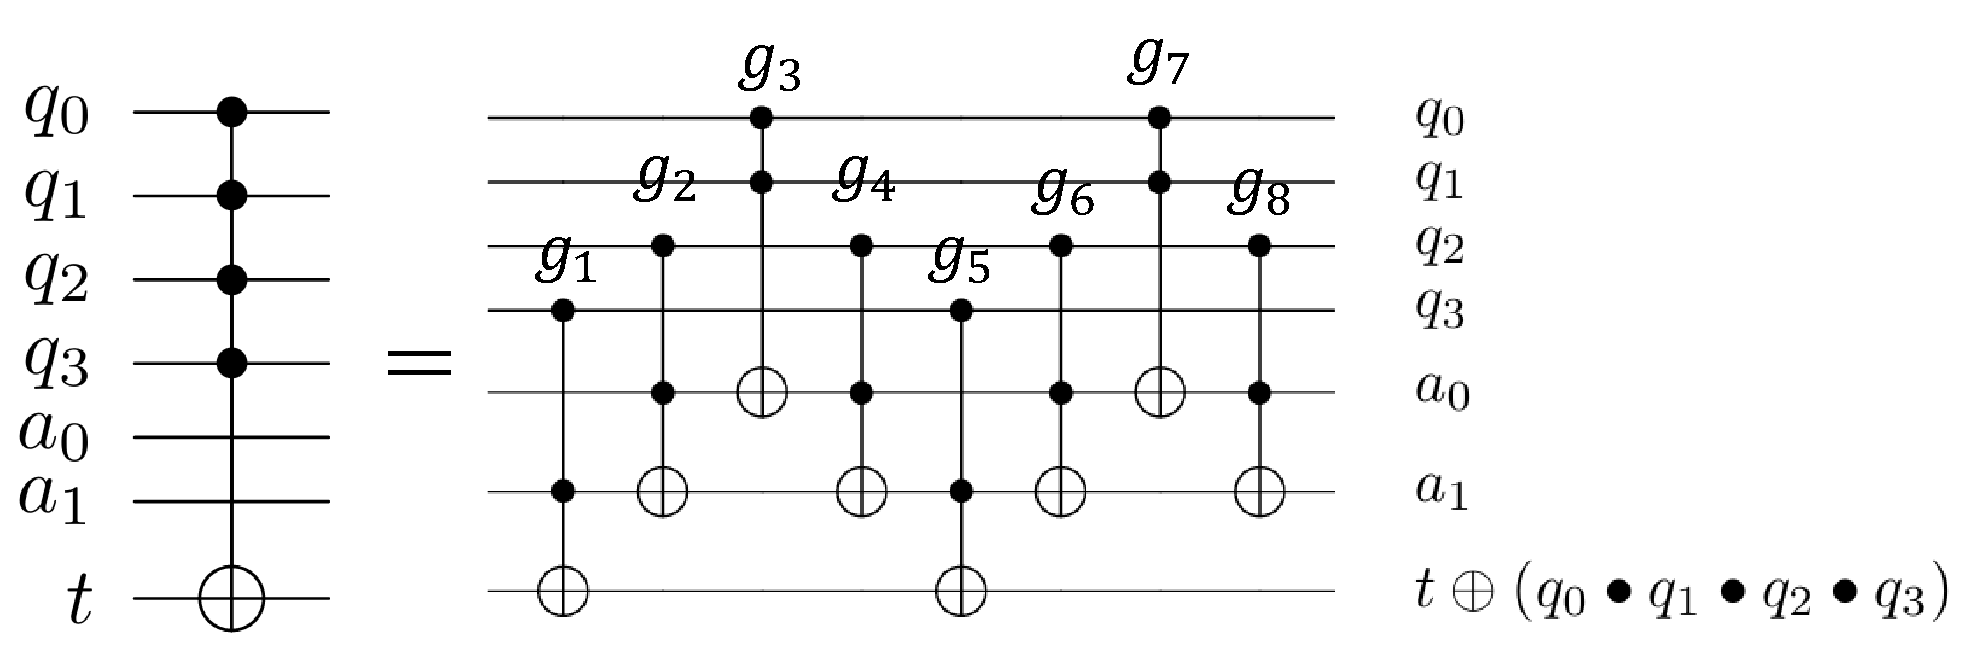
\includegraphics[width=0.95\linewidth]{img/barenco.pdf}
\caption{Example of decomposition of MCT gate into Toffoli gates}
\label{barenco}
\end{figure}
In Figure~\ref{barenco}, the MCT gate is decomposed into Toffoli gates using ancilla qubits $a_{0} and a_{1}$ with undefined values.
If the number of control bits of the MCT gate is $c$, the MCT gate can be decomposed into $4(c-2)$ Toffoli gates using $c-2$ ancilla qubits with undefined values\cite{barenco1995elementary}.
In the example in Figure~\ref{barenco}, the MCT gate with 4 control bits is decomposed into 8 Toffoli gates using 2 ancilla qubits with undefined values.

\begin{table}
  \begin{tabular}{c|c|c|c}
    \hline
    Method   & Ref                             & \#Aux  & T-depth \\\hline
    Method~1 & \cite{abdessaied2016technology} & $c-2$ & $4(c-1)$\\\hline 
    Method~2 & \cite{abdessaied2016technology} & $<c-2$ & $8(c-1)-8+4=8c-20$ \\\hline
    Method~3 & \cite{baker2019decomposing}     & $2 to c-3$ & $6\cdot (2 \cdot log c-3$\\\hline
    Method~4 & \cite{niemann2019t}             & $c-2$ & $4\lceil log2(c) \rceil - 1$\\\hline            
  \end{tabular}
  \caption{Summary MCT Decomposition Methods}
  \label{decomp-table}
\end{table}

\section{MCT Decomposition}
In this chapter, we explain the existing \bout{decomposition method\cite{abdessaied2016technology,baker2019decomposing,niemann2019t}} of MCT gates. We denote the number of control bits of each MCT gate as $c$. They are summarized in Table~\ref{decomp-table}. {\it Method} displays how the method is referred to in this paper, {\it Ref} is the source citation for the method, {\it \#Aux} is the number of ancilla qubits available, and {\it T-depth} is the worst case T-depth for each method. 

In the interest of space, we only explain the decomposition method in \cite{abdessaied2016technology}, hereafter called Method~1. This should give an intuitive feel for how such a decomposition can reduce the T-depth, and more details for each method are available in the associated citation.

\bout{Method~1} uses $c-2$ ancilla qubits with indefinite values to reduce the T-depth of the method \cite{barenco1995elementary} that decomposes MCT gates into Toffoli gates.

In Method~1, the T-depth is reduced by replacing Toffoli gates with out-of-phase $CCiZ, CCi\omega Z$ gates, both of which can be implemented in T-depth of 1 with no additional ancilla. The result is depicted in Fig.~\ref{barenco_iz_to_iomegaz}.

\begin{figure}[tbp]
\centering
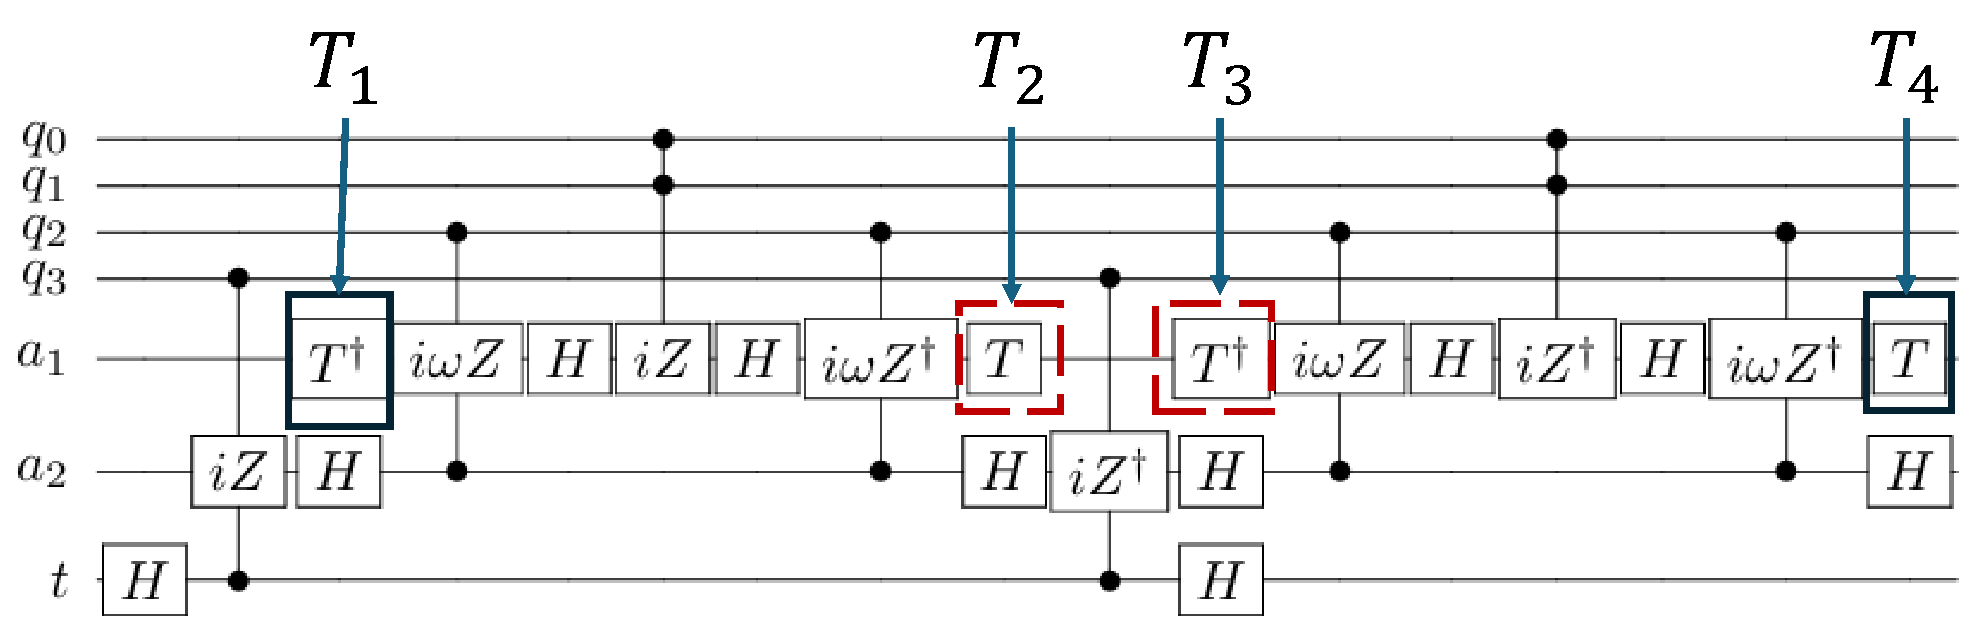
\includegraphics[width=0.95\linewidth]{img/barenco_iz_to_iomegaz.pdf}
\caption{Replacement of Toffoli gates in a MCT gate decomposition with $CCiZ$ and $CCi\omega Z$ gates.}

\label{barenco_iz_to_iomegaz}

\end{figure}
